\newpage
\mysection{Anhang}

\mysubsection{Configure bazel for Tensorflow}

\begin{lstlisting}[caption=Configure bazel for Tensorflow, label=list:configure_bazel, language=bash]
	$ cd tensorflow  # cd to the top-level directory created
	$ ./configure
	Please specify the location of python. [Default is /usr/bin/python]: /usr/bin/python3.6
	Found possible Python library paths:
	  /usr/local/lib/python3.6/dist-packages
	  /usr/lib/python3.6/dist-packages
	Please input the desired Python library path to use.  Default is [/usr/lib/python3.6/dist-packages]
	Using python library path: /usr/local/lib/python3.6/dist-packages
	Do you wish to build TensorFlow with MKL support? [y/N]
	No MKL support will be enabled for TensorFlow
	Please specify optimization flags to use during compilation when bazel option "--config=opt" is specified [Default is -march=native]:
	Do you wish to use jemalloc as the malloc implementation? [Y/n]
	jemalloc enabled
	Do you wish to build TensorFlow with Google Cloud Platform support? [y/N]
	No Google Cloud Platform support will be enabled for TensorFlow
	Do you wish to build TensorFlow with Hadoop File System support? [y/N]
	No Hadoop File System support will be enabled for TensorFlow
	Do you wish to build TensorFlow with the XLA just-in-time compiler (experimental)? [y/N]
	No XLA support will be enabled for TensorFlow
	Do you wish to build TensorFlow with VERBS support? [y/N]
	No VERBS support will be enabled for TensorFlow
	Do you wish to build TensorFlow with OpenCL support? [y/N]
	No OpenCL support will be enabled for TensorFlow
	Do you wish to build TensorFlow with CUDA support? [y/N] Y
	CUDA support will be enabled for TensorFlow
	Do you want to use clang as CUDA compiler? [y/N]
	nvcc will be used as CUDA compiler
	Please specify the Cuda SDK version you want to use, e.g. 7.0. [Leave empty to default to CUDA 8.0]: 8.0
	Please specify the location where CUDA 8.0 toolkit is installed. Refer to README.md for more details. [Default is /usr/local/cuda]:
	Please specify which gcc should be used by nvcc as the host compiler. [Default is /usr/bin/gcc]:
	Please specify the cuDNN version you want to use. [Leave empty to default to cuDNN 6.0]: 6
	Please specify the location where cuDNN 6 library is installed. Refer to README.md for more details. [Default is /usr/local/cuda]:
	Please specify a list of comma-separated Cuda compute capabilities you want to build with.
	You can find the compute capability of your device at: https://developer.nvidia.com/cuda-gpus.
	Please note that each additional compute capability significantly increases your build time and binary size.
	[Default is: "3.5,5.2"]: 3.0
	Do you wish to build TensorFlow with MPI support? [y/N]
	MPI support will not be enabled for TensorFlow
	Configuration finished
\end{lstlisting}

\newpage
\begin{sidewaysfigure}
\mysubsection{Mobile Application Architecture in the form of a Class Diagram}
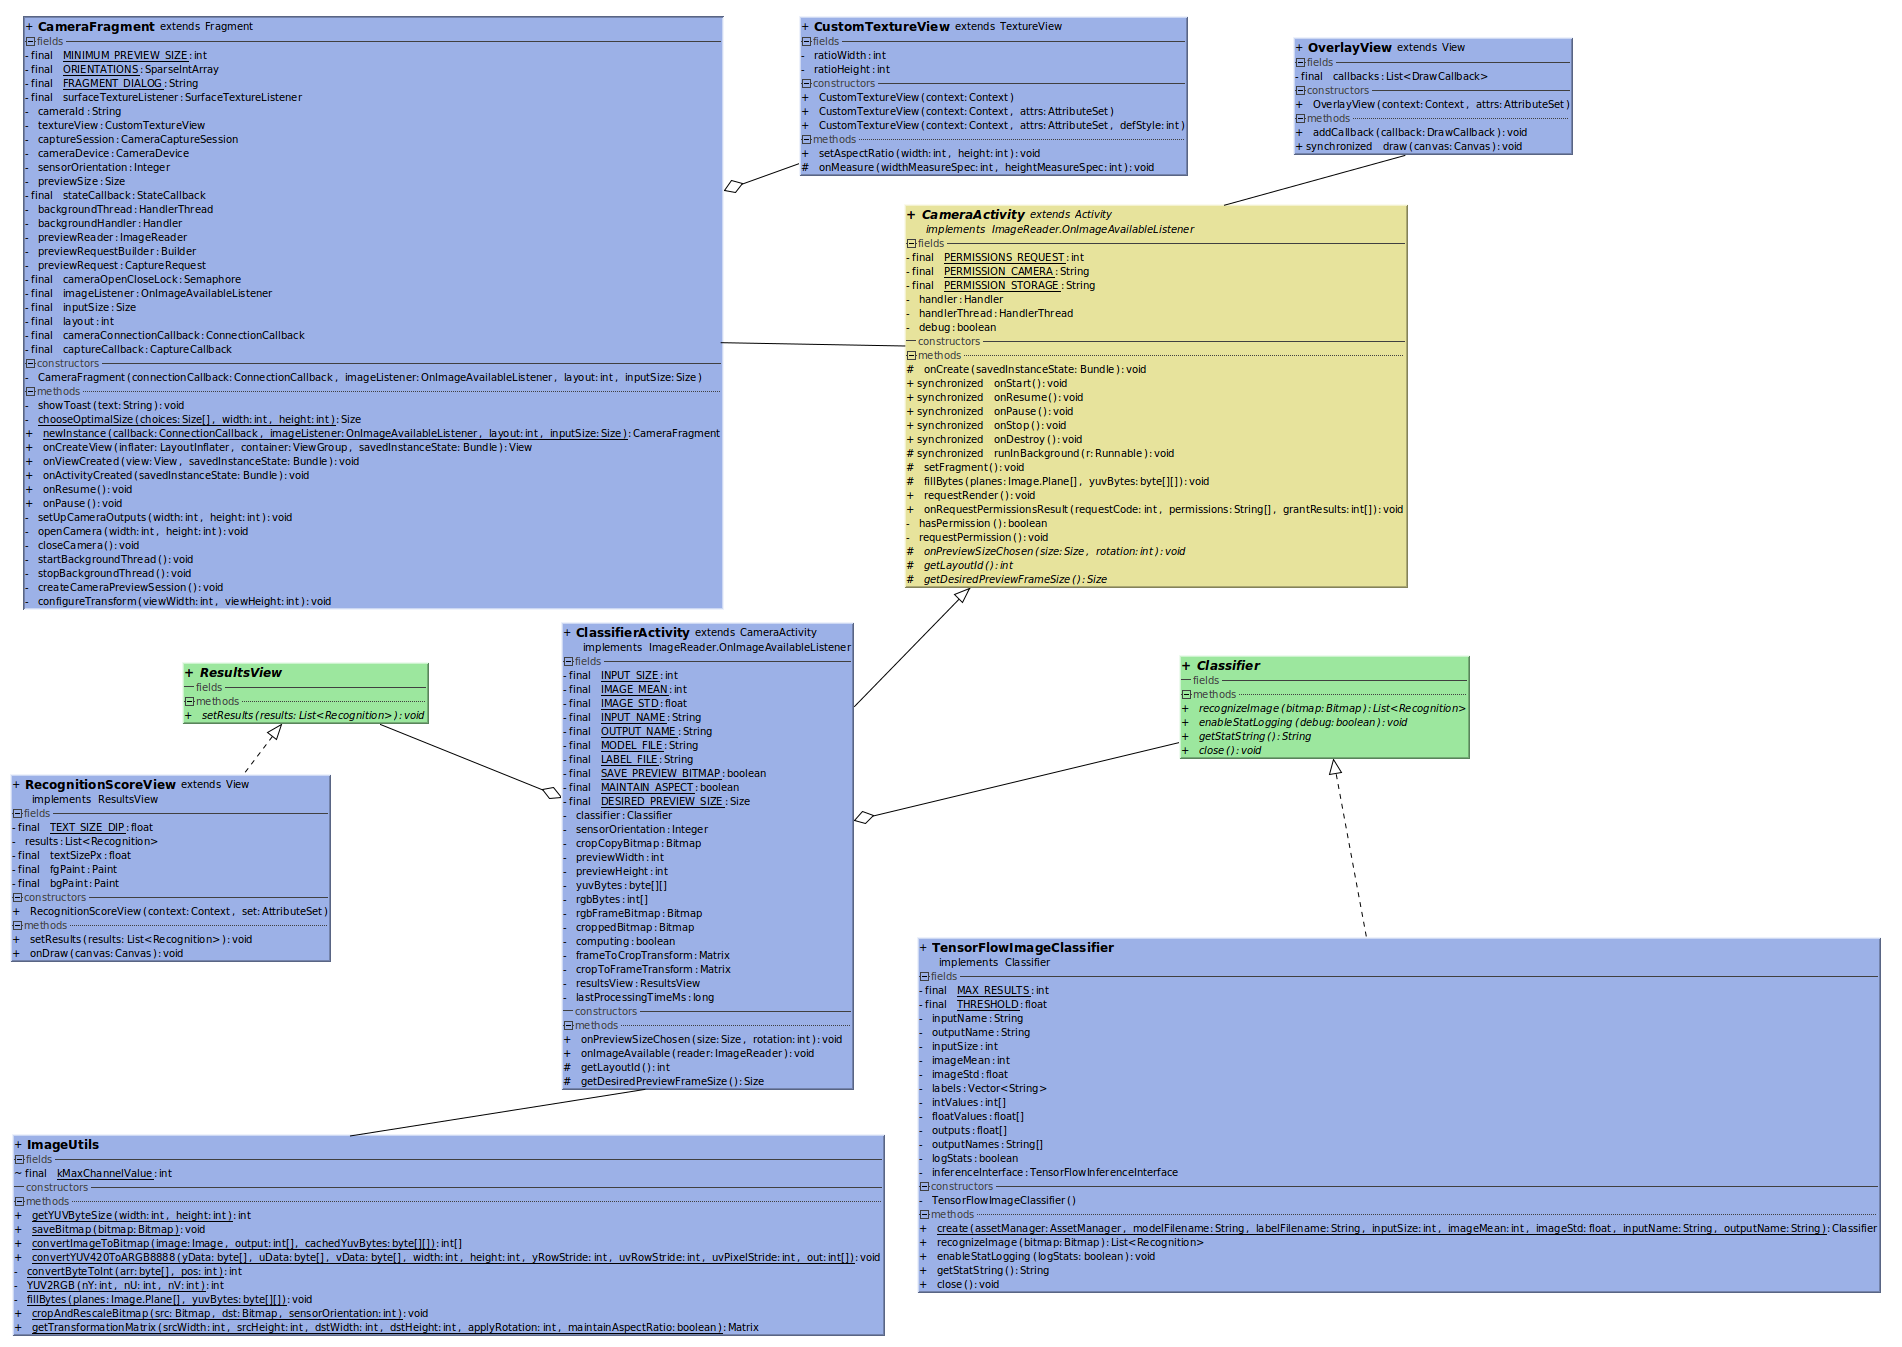
\includegraphics[width=0.95\textwidth]{includes/ClassDiagram}
\end{sidewaysfigure}
